\documentclass[11pt]{article}

\usepackage[a4paper,margin=2.2cm]{geometry}
\usepackage{graphicx}
\usepackage{booktabs}
\usepackage{microtype}
\usepackage{xspace}
\usepackage{placeins}
\usepackage{array}
\usepackage[numbers,sort&compress]{natbib}
\usepackage[colorlinks=true,allcolors=blue]{hyperref}

\newcommand{\ramplotr}{\textsc{RamplotR}\xspace}
\newcommand{\degree}{^\circ}

\title{\ramplotr: residue-centred exploration and comparison of protein backbone conformation}
\author{Cedric Hermans\\
Howest University of Applied Sciences, Belgium\\
\href{https://orcid.org/0000-0002-9310-1876}{ORCID: 0000-0002-9310-1876}}
\date{Preprint draft -- October 2026}

\begin{document}
\maketitle

\begin{abstract}
Ramachandran plots remain a standard representation of protein backbone geometry, but practical interpretation often requires moving between a plot, sequence position, molecular viewer, model-confidence information and structurally related models. We present \ramplotr, an open-source R/Shiny application centred on residue-level exploration of backbone conformation in experimental and predicted protein structures. A selected residue remains linked across the Ramachandran plot, sequence navigator, residue table and three-dimensional structure. The same residue-centred workflow extends to pairwise conformational comparison, prediction ensembles, structure groups and experimentally determined counterparts of predicted models.

\ramplotr separates exploratory density visualization from standard Ramachandran validation. Native density regions can be inspected against several bundled reference datasets, while a parallel six-class Rama8000 evaluation reproduces the current cctbx/Phenix Favored, Allowed and Outlier definitions. Backbone calculations were evaluated against Bio3D and independently generated wwPDB validation reports. Across five deposited structures representing X-ray crystallography, cryo-EM and NMR, all 3,718 eligible matched $\phi/\psi$ pairs agreed with wwPDB-reported values to within $0.055\degree$, and all 3,718 Rama8000 classifications matched the corresponding official wwPDB categories.

For predicted structures, \ramplotr keeps pLDDT and PAE separate from stereochemical validation and can compare independently generated AlphaFold, AlphaFold 3, ColabFold or ESMFold models using circular backbone statistics. Pairwise and group workflows expose local conformational shifts directly in $\phi/\psi$ space and link them back to aligned residues in three dimensions. The comparison workflow additionally reports sequence identity and coverage, paired prediction confidence when available, and local non-water hetero-residue context as separate evidence layers. \ramplotr is intended as a focused exploratory and reporting workbench that complements, rather than replaces, comprehensive structure-validation and model-building suites.
\end{abstract}

\section{Introduction}

Backbone $\phi$ and $\psi$ torsion angles provide a compact description of local protein conformation and remain a standard way to inspect stereochemical plausibility \citep{Ramachandran1963}. Contemporary structure-validation workflows use residue-specific reference distributions together with complementary model-quality criteria, as implemented in MolProbity, Phenix and wwPDB validation \citep{Williams2018,Liebschner2019,Gore2017}. Whole-model measures such as Rama-Z address the related question of whether the overall Ramachandran distribution of a model is plausible \citep{Sobolev2020}.

Interactive structure analysis is rarely limited to a single validation plot. Coot links validation findings to model-building operations \citep{Emsley2010}; Iris presents multiple residue-level validation signals in a compact interactive representation \citep{Rochira2021}; and the SWISS-MODEL Structure Assessment server links sequence, three-dimensional structure, Ramachandran and MolProbity results, model-quality estimates and model-to-reference comparisons \citep{Waterhouse2024}. PDBe provides archive-level access to coordinates, annotations and wwPDB validation information for deposited structures \citep{Varadi2022PDBe}. These tools establish that linked residue navigation and interactive Ramachandran visualization are themselves not novel.

At the same time, predicted structures have become a routine starting point for structural analysis. AlphaFold 2, AlphaFold 3 and ESMFold provide complementary routes to predicted structures \citep{Jumper2021,Abramson2024,Lin2023}, while AlphaFold DB provides large-scale access to predicted models \citep{Varadi2024}. Predicted structures introduce additional questions that are not captured by a single confidence value: whether independent samples agree on a local backbone state, whether an unusual conformation occurs in an experimental counterpart, and whether a conformational difference between two structures is localized to particular aligned residues.

\ramplotr was developed around these residue-level questions. Its emphasis is not comprehensive validation, refinement or archive annotation. Instead, backbone conformation is used as the common coordinate system for moving between sequence, three-dimensional context, standard validation, prediction confidence and related structures. Pairwise comparisons retain aligned residue identity while reporting wrapped $\Delta\phi/\Delta\psi$ values; prediction ensembles summarize circular angular variation and confidence across independent models; structure groups can be compared residue by residue; and predicted models can search for candidate experimental counterparts and open them directly in the same comparison workflow. The application can run as a conventional R/Shiny application \citep{Shiny2026} or as a Shinylive/webR browser deployment \citep{Shinylive2026}.

This paper describes the current implementation and validates the numerical backbone and standard Rama8000 calculations against independent sources. The contribution is a focused conformation-centred workflow rather than a new general-purpose validation metric.

\section{Software design and workflow}

\subsection{Structure input and backbone geometry}

\ramplotr accepts PDB accessions and uploaded PDB or mmCIF coordinate files. Coordinate parsing is performed with Bio3D \citep{Grant2006}; public deposited structures are obtained from the Protein Data Bank \citep{Burley2019}. Residues are identified by chain, residue number and insertion code. For alternate conformations, unlabelled atoms are preferred, followed by alternate A.

Backbone $\phi/\psi$ angles are calculated from N, C$\alpha$ and C coordinates. A torsion is evaluated across consecutive residue records only when they belong to the same chain and the intervening C--N distance is compatible with peptide continuity (1.0--1.9~\AA). Missing atoms and chain breaks therefore produce missing torsions rather than artificial angles. The preceding peptide $\omega$ angle is retained where available so that proline residues can be separated into cis- and trans-proline classes for standard validation.

\subsection{Native density exploration and Rama8000 standard validation}

\ramplotr deliberately exposes two distinct views of Ramachandran geometry.

The native density view supports several bundled reference datasets and residue-aware evaluation of general, glycine, proline and pre-proline residues. It reports the four \ramplotr density-region labels Favoured, Allowed, Generously allowed and Not allowed. The selected plotting background is independent of the residue-specific classification calculation, allowing alternative density distributions to be explored without changing the displayed residue identity.

For standard validation, \ramplotr independently implements the six-class Rama8000 model used by current cctbx/Phenix validation: General, Gly, cis-Pro, trans-Pro, pre-Pro and Ile/Val \citep{Williams2018,Liebschner2019}. The corresponding 180$\times$180 reference score tables are evaluated with periodic bilinear interpolation and the class-specific Favored, Allowed and Outlier thresholds used by cctbx. The reference tables are vendored with their upstream revision and license provenance. Rama8000 results do not depend on the selected native \ramplotr background.

The two outputs are intentionally kept separate in the interface and exports. In particular, the native label Not allowed is not treated as a synonym for a Rama8000/wwPDB Outlier.

\subsection{Residue-centred interactive exploration}

The central interaction in \ramplotr is residue selection (Figure~\ref{fig:overview}). Selecting a point in the Ramachandran plot identifies the same residue in the table, sequence navigator and NGL molecular viewer \citep{Rose2015}; selection from the sequence or three-dimensional structure performs the inverse linkage. The molecular viewer then focuses on the selected local structural environment.

The sequence navigator uses actual PDB residue numbers and insertion codes rather than an interface-specific sequential index. Native density state, Rama8000 validation and, when applicable, prediction confidence are represented with separate visual channels. A residue inspector summarizes the available evidence without collapsing it into a composite score. It can identify, for example, a Rama8000 outlier, proximity to a native density boundary, prediction confidence, attached official wwPDB annotations and nearby non-water hetero residues. If no unusual signal is present, the interface reports this explicitly rather than generating an artificial warning.

\begin{figure}[ht]
\centering
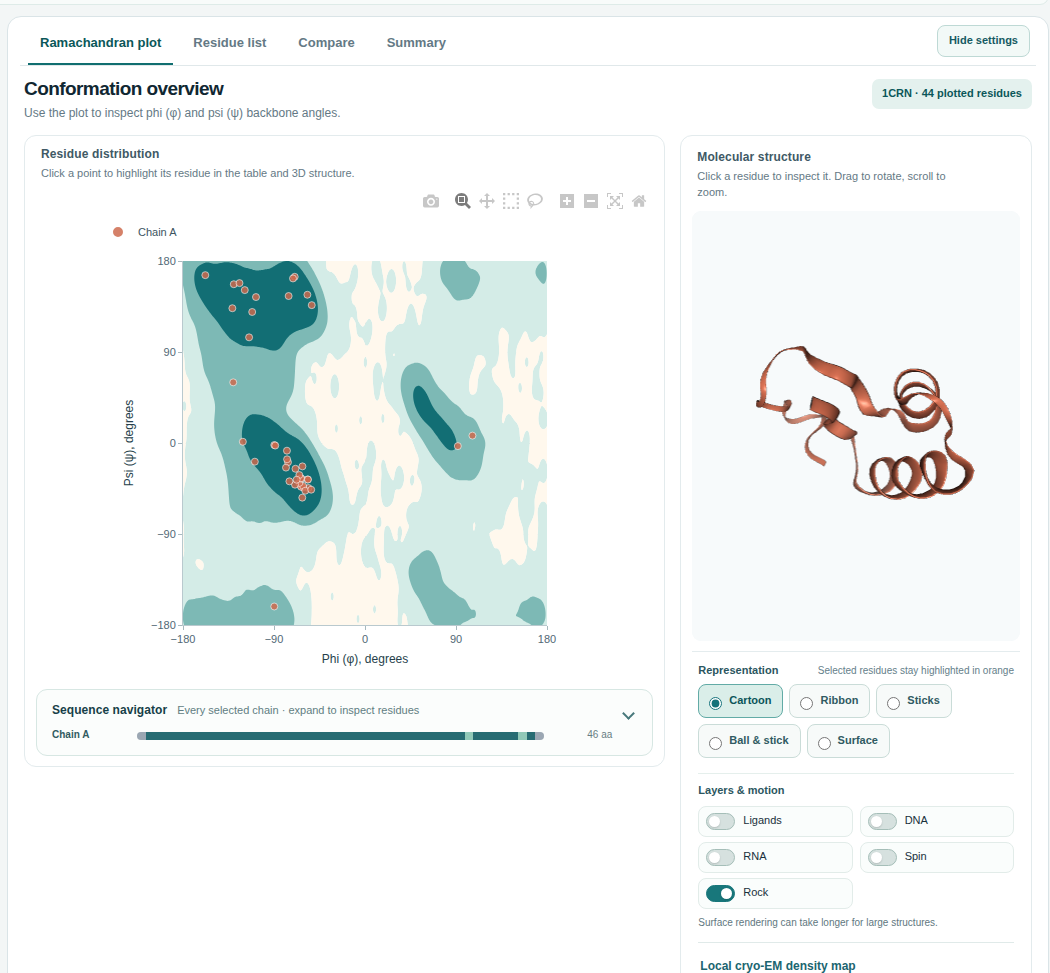
\includegraphics[width=0.94\linewidth]{../docs/screenshots/overview.png}
\caption{\ramplotr analysis workspace. Ramachandran geometry, sequence position, residue information and the molecular structure are linked through residue identity, allowing a point on the plot to be inspected directly in structural context.}
\label{fig:overview}
\end{figure}

\subsection{Predicted structures and model confidence}

Predicted structures can be loaded from local files or retrieved from AlphaFold DB \citep{Varadi2024}. For AlphaFold 2/ColabFold and ESMFold models, pLDDT can be interpreted from the coordinate B-factor field only when prediction provenance is explicitly declared. Experimental B factors are never automatically interpreted as confidence scores. AlphaFold 3 confidence JSON can provide per-atom pLDDT and token-level PAE when it maps consistently to the supplied coordinates \citep{Abramson2024}.

pLDDT is shown as a residue-level signal in the sequence navigator and detail view, while PAE can be displayed as a heatmap linked to residue selection. These measures remain separate from stereochemical validation: high pLDDT does not make a Rama8000 outlier acceptable, and low confidence does not itself establish a geometric error.

\subsection{Conformational comparison}

A second structure can be loaded for direct comparison. Selected protein chains are aligned by amino-acid sequence rather than residue number, preserving substitutions, insertions and deletions. For every aligned residue pair with finite backbone angles, $\Delta\phi$ and $\Delta\psi$ are wrapped across the $-180\degree/180\degree$ boundary. A combined local displacement,
\[
d_{\phi\psi}=\sqrt{(\Delta\phi)^2+(\Delta\psi)^2},
\]
is used only as a navigation and ranking measure; it is neither a Cartesian structural distance nor a significance score.

The Conformational Change Explorer displays aligned residues as a compact track ordered along the sequence. Selecting a residue from this track, the comparison table, either Ramachandran representation or either three-dimensional structure selects the aligned pair everywhere. The paired molecular view is superposed on the selected chains and can focus on both positions simultaneously. The aligned-angle plot uses the same selected density background as the individual Ramachandran plot. Primary and comparison roles can be exchanged without reloading either structure while preserving structure-specific chain and model choices.

Because local structural differences are meaningful only when the sequence correspondence is credible, the comparison summary reports sequence identity and aligned coverage for both selected chains and flags low-identity or low-coverage comparisons for cautious interpretation. When both structures carry declared prediction confidence, pLDDT is retained for both aligned residues and signed $\Delta$ pLDDT is reported independently from backbone displacement. The selected-pair inspector also reports nearby non-water hetero residues for both structures using a fixed local distance search. This proximity is presented as structural context only and is not interpreted automatically as biochemical binding or functional equivalence.

For predicted models, candidate experimentally determined counterparts can be identified through sequence search against experimental PDB polymer entities. Candidate method and resolution are shown with a link to the corresponding PDBe entry, and a selected candidate can be opened directly in the linked comparison workflow. Sequence similarity identifies a candidate counterpart; it is not treated as evidence that both structures represent the same biochemical state.

\subsection{Prediction and structure ensembles}

Multi-model coordinate files can be summarized using residue-wise circular means and circular standard deviations for $\phi/\psi$. Independently generated prediction models can additionally be analysed as prediction ensembles. AlphaFold 2/ColabFold, ESMFold and compatible prediction files retain per-residue pLDDT; AlphaFold 3 sample sets are paired with their corresponding confidence JSON by sample identity rather than upload order. Model-level AlphaFold 3 quantities such as pTM, ipTM and ranking score remain model-level provenance and are not combined into the residue variability measure.

The ensemble view reports how many models contain each residue, circular angular spread, Rama8000 category consistency and confidence variation where available. Residue-level ensemble disagreement can be returned to the same shared inspector used for single-structure and pairwise evidence, allowing a locally variable prediction to be examined directly in sequence and three-dimensional context. Prediction-model disagreement is described as prediction uncertainty or heterogeneity, not as experimental evidence of molecular dynamics.

For biologically defined sets of structures, such as apo versus ligand-bound or wild-type versus mutant, \ramplotr can align uploaded structures to a common reference chain and compare group-level circular backbone statistics. Coverage and within-group dispersion remain visible alongside the between-group conformational effect so that a large shift supported by sparse or internally heterogeneous data is not presented as equivalent to a reproducible group difference.

\subsection{External validation and reproducible output}

For deposited experimental structures, users can optionally attach the official wwPDB validation XML for the corresponding structure and model \citep{Gore2017}. Matching uses model, chain, residue number, insertion code and residue identity. Imported annotations remain explicitly external evidence and do not modify either native density results or the independently calculated Rama8000 result.

Interactive analyses can export filtered residue and comparison tables, publication-oriented figures and HTML reports with analysis settings and provenance. An offline batch interface applies the same backbone and classification functions to local files. The Shinylive build executes the R application in the browser through webR, offering a no-install route while retaining native R execution for local and scripted analyses.

\section{Validation}

\subsection{Backbone-angle calculations}

The custom backbone calculation was cross-checked against Bio3D \citep{Grant2006} using the small 1CRN structure and the substantially larger 6VXX structure. Residues were matched by structural identifiers and compared only where both implementations returned finite angles. The largest observed absolute difference was approximately $1.1\times10^{-11}\,^\circ$, consistent with floating-point-level numerical differences for the tested cases.

A second independent comparison used official wwPDB validation reports. Five deposited structures were selected purposively to exercise different experimental modalities and edge cases: X-ray crystallography (1CRN, 1UBQ and outlier-containing 2DQ4), a large cryo-EM structure (6VXX), and an NMR ensemble (model 1 of 1D3Z). This is a functional validation set rather than a random sample of the PDB. The repository pins the coordinate and validation-report sources together with their hashes. \ramplotr-computed torsions were joined to official wwPDB residues by model, chain, residue number, insertion code and residue identity, and angle differences were evaluated circularly.

\subsection{Direct Rama8000 comparison}

The same matched residues were evaluated using the six-class Rama8000 implementation. Favored, Allowed and Outlier were compared directly with the corresponding official wwPDB Ramachandran category. No mapping of the native four \ramplotr density regions was used. The validation workflow pins both source hashes and expected category counts and fails if the same source files no longer reproduce the expected Rama8000 result.

\section{Results}

\subsection{Backbone-angle and standard-category agreement}

Across the five-structure corpus, all 3,718 eligible finite $\phi/\psi$ pairs matched an independently reported wwPDB residue and agreed with the report values to within $0.055\degree$ (Table~\ref{tab:wwpdb}). The official XML reports angles to one decimal place, consistent with the approximately $0.05\degree$ residual differences.

The Rama8000 comparison also matched exactly: all 3,718 comparable residues received the same Favored, Allowed or Outlier category as the official wwPDB report. In the outlier-containing 2DQ4 structure, all seven official Ramachandran outliers were independently classified as Rama8000 Outlier by \ramplotr.

\begin{table}[ht]
\centering
\caption{Independent comparison with official wwPDB validation reports. Rama8000 agreement is a direct category comparison; native \ramplotr density regions are not involved.}
\label{tab:wwpdb}
\small
\begin{tabular}{llrrrr}
\toprule
Structure & Method & Angle pairs & Max. diff. ($^\circ$) & Rama8000 matches & Agreement\\
\midrule
1CRN & X-ray & 44/44 & 0.052 & 44/44 & 100\%\\
1UBQ & X-ray & 74/74 & 0.054 & 74/74 & 100\%\\
6VXX & cryo-EM & 2,844/2,844 & 0.055 & 2,844/2,844 & 100\%\\
2DQ4 & X-ray & 682/682 & 0.055 & 682/682 & 100\%\\
1D3Z & NMR, model 1 & 74/74 & 0.055 & 74/74 & 100\%\\
\midrule
Total & & 3,718/3,718 & $\leq0.055$ & 3,718/3,718 & 100\%\\
\bottomrule
\end{tabular}
\end{table}

\section{Discussion}

The strongest reason to use \ramplotr is not that it displays a Ramachandran plot or links a selected residue to a molecular viewer; both capabilities exist in mature structural-biology software. MolProbity/Phenix provide substantially broader reference-grade validation \citep{Williams2018,Liebschner2019}, Coot integrates validation with model building \citep{Emsley2010}, Iris provides multi-metric residue validation \citep{Rochira2021}, and the SWISS-MODEL Structure Assessment server combines stereochemistry, sequence, three-dimensional visualization, quality estimates and model-to-reference benchmarking \citep{Waterhouse2024}. \ramplotr instead concentrates on local backbone conformation as the common object of exploration across experimental structures, predictions and sets of related models.

This focus becomes most distinct when the scientific question is comparative rather than simply diagnostic. In pairwise comparison, an aligned residue can be followed simultaneously through both $\phi/\psi$ positions and both superposed three-dimensional structures, while sequence identity, chain coverage, local structural context, Rama8000 state and prediction-confidence differences remain visible as separate evidence. Prediction ensembles retain circular backbone spread, confidence variation and standard-validation state for each residue across independently generated samples. A predicted model can search for experimental counterparts and move directly from sequence similarity to the same local comparison workflow. Structure-group comparison extends the same representation to biologically defined sets. These workflows are intended to answer questions such as whether a local backbone state is reproduced across prediction samples, whether a predicted conformation occurs in an experimental structure, and which aligned residues account for a conformational difference between two structural states.

The separation of evidence types is an important design principle. Rama8000 supplies the standard Favored/Allowed/Outlier result; native density references remain available for exploratory visualization; pLDDT and PAE describe prediction confidence; official wwPDB reports provide independent deposited-structure evidence; and group or ensemble variation describes the supplied set of models. These signals are shown together but are not combined into a single quality score.

The independent validation supports the numerical foundations of this workflow. The angle calculations agree with both Bio3D and wwPDB-derived values, while the exact 3,718/3,718 Rama8000 category agreement demonstrates that the standard classification reproduces the pinned official validation corpus. This result should not be generalized into a claim that \ramplotr replaces complete wwPDB or MolProbity validation: clashes, rotamers, covalent geometry, experimental data quality and whole-model measures remain outside the scope of the Rama8000 calculation.

Several limitations remain. The independent validation corpus contains only five purposively selected structures and is designed as a functional regression set rather than a population-level study. Only model 1 of the NMR example is used in the independent wwPDB comparison. Prediction-ensemble variation depends on which models, seeds and confidence files are supplied and must not be interpreted as molecular dynamics. Sequence-similar experimental counterparts can differ in ligand state, construct, oligomerization or functional state. The combined pairwise $\phi/\psi$ displacement is a navigation aid rather than a calibrated biological effect size. No formal user study has been performed, so the paper does not claim quantitatively superior usability over existing structure-analysis environments.

\section{Availability and reproducibility}

\ramplotr is available under the MIT license at
\url{https://github.com/BiKC/RamplotR}. A browser version is available at
\url{https://bikc.be/RamplotR/}. The software revision described by this draft is repository \texttt{main} at commit \texttt{6d1e4e95cdf5df4ae63bdbeccb4a6eeb7af41a1a}; manuscript development is maintained on the \texttt{arxiv-preprint} branch.

The repository contains the pinned independent wwPDB validation manifest, exact source hashes, angle baselines and Rama8000 category baselines. Continuous integration reruns the scientific regression suite, independent wwPDB comparison, browser workflows and structure-validation benchmarks. Prediction-ensemble and comparison exports retain model identities and analysis provenance needed to reproduce a reported result.

\section{Conclusion}

\ramplotr is a residue-centred workbench for exploring protein backbone conformation across experimental structures and predictions. Its role is not to replace comprehensive validation suites, but to make local $\phi/\psi$ geometry directly navigable together with sequence, three-dimensional context, standard Rama8000 validation, prediction confidence and corresponding residues in related structures. Independent comparisons support both the backbone-angle implementation and the standard Ramachandran categories. The comparison, ensemble and experimental-counterpart workflows extend that validated foundation from single-structure inspection to the analysis of local conformational differences between structures and predictions.

\section{Author contributions}

Cedric Hermans: software development, methodology, validation, visualization, documentation and manuscript draft. The author list and contribution statement are provisional and should be reviewed before submission.

\section{Competing interests}

The author declares no competing interests.

\bibliographystyle{plainnat}
\bibliography{references}

\end{document}
